%======================================================================
\NEWSEC
%======================================================================


\subsection{\ssRecentGravity}



%----------------------------------------------------------------------
%  Scalable AMR Gravity
%  
%
\begin{frame}[fragile,label=ss-recent-gravity] 
\secframetitle{\ssRecentGravity}
\framesubtitle{Current status}
\begin{itemize}
   \item Gravity available previously
\begin{itemize}
   \item        CG, BiCG-STAB Krylov solvers
 \item       $O(N^{4/3})$ for $3D$
\item       not feasible for large problems
\end{itemize}
   \item Scalable unigrid gravity available now
\begin{itemize}
   \item        MG0: unigrid multigrid V-cycle solver
\item         efficiency $O(1/\log P)$ for $N \rightarrow \infty$, $N/P = $const
\end{itemize}
   \item  Scalable AMR gravity soon
\begin{itemize}
\item HG [Reynolds] BiCG-STAB + MG-like preconditioner
\item         \textit{almost} working (one bug left!)
\item          high quality solution even at level boundaries
\item         expected higher performance than MG0
\item          (provided not too deep AMR)
\end{itemize}
\end{itemize}
\end{frame}
%
%----------------------------------------------------------------------
% Gravity solver in Enzo-P
%
\begin{frame}[fragile,label=ss-recent-gravity] 
\secframetitle{\ssRecentGravity}
\framesubtitle{Gravity solver in Enzo-P}
   Enzo's CIC PM self-gravity is split between multiple Enzo-P ``Method''s
\begin{itemize}
\item \greencode{EnzoMethodPmDeposit}
\begin{itemize}
\item        compute \code{"density\_total"} field
\item        \code{"density"} field + \code{"dark"} particle density
\item        Enzo: \bluecode{PrepareDensityField}
\end{itemize}
\item \greencode{EnzoMethodGravity}
\begin{itemize}
\item        compute potential from \code{"density\_total"}
\item        flexible linear Solvers: \code{"cg"}, \code{"mg0"}, etc.
\item        computes acceleration given potential
\item        Enzo: \bluecode{SolveForPotential, ComputeAccelerations}
\end{itemize}
\item \greencode{EnzoMethodPmUpdate}
\begin{itemize}
\item        update particle positions
\item        KDK method
\item        Enzo: \bluecode{UpdateParticlePositions}
\end{itemize}
\end{itemize}
\end{frame}


%    Cello handles relocating particles as well as ghost zone refresh
%----------------------------------------------------------------------
% Scalable AMR Gravity
\begin{frame}[fragile,label=ss-recent-gravity] 
\secframetitle{\ssRecentGravity}
\framesubtitle{Sample gravity parameter file excerpt}
\small
\begin{tabbing}
\code{xxxx}\=\code{xxxx}\=\code{xxxx}\= \kill
\> \code{Method \{ } \\
\> \>  \code{list = [ "pm\_deposit", "gravity", "ppm", "pm\_update" ]; } \\
\> \>  \code{gravity \{  solver = "MG"; \} } \\
\> \} \\
\\
\> \code{Solver \{ } \\
\> \> \code{list = ["MG","P1","C","P2"]; } \\
\> \> \code{MG \{ } \\
\> \> \> \code {type = "mg0"; } \\
\> \> \> \code {local = true; } \\
\> \> \code{\} } \\
\> \> \vdots \\
\> \code{     \} }
\end{tabbing}
\end{frame}
%
%----------------------------------------------------------------------
%
%  Scalable AMR Gravity
\begin{frame}[fragile,label=ss-recent-gravity] 
\secframetitle{\ssRecentGravity}
\framesubtitle{Parallel scaling test problem}

\textbf{We tested scalability of a recently implemented gravity solver}
\begin{minipage}{1.5in}
  \vspace{0.2in}
  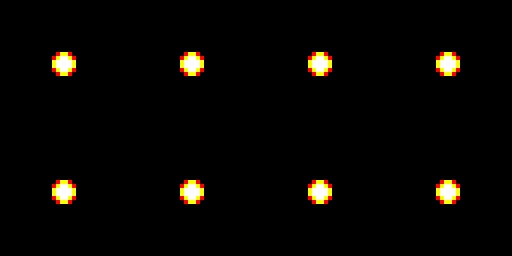
\includegraphics[width=1.5in]{de.png} \ \\
  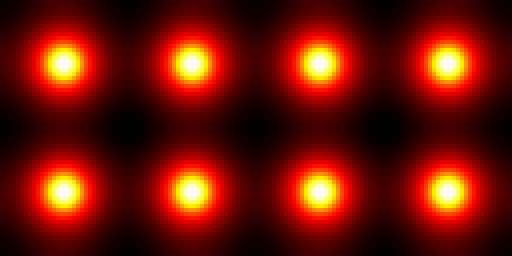
\includegraphics[width=1.5in]{po.png} \ \\
  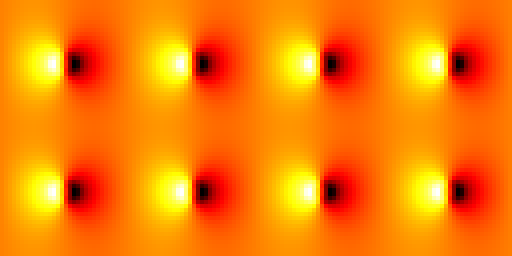
\includegraphics[width=1.5in]{axz.png}
\end{minipage} \
\begin{minipage}{2.75in}
\centerline{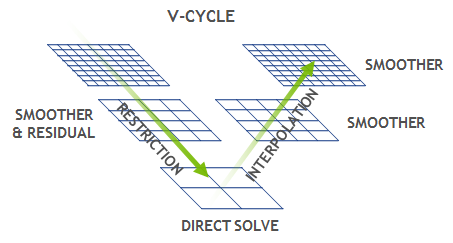
\includegraphics[width=1.5in]{hpgmg_v_cycle.png}}
  \begin{itemize}
  \item ``array of collapsing spheres'' problem
  \item varied both block size and problem size
  \item multigrid V-cycle solve (uniform-mesh)
  \item debugging scalable AMR gravity
    \begin{itemize}
      \item Reynolds ``HG'' algorithm
    \item BiCG-STAB Krylov solver
    \item multigrid-based preconditioner
    \end{itemize}
  \end{itemize}
\end{minipage}
\end{frame}
%  Parallel scaling test problem
%
%    [ IMAGE ] density
%    [ IMAGE ] potential
%    [ IMAGE ] acceleration
%    [ IMAGE ] tracer particles
%
%----------------------------------------------------------------------
% Scalable AMR Gravity
\begin{frame}[fragile,label=ss-recent-gravity] 
\secframetitle{\ssRecentGravity}
\framesubtitle{Gravity weak scaling}
  \begin{center}
    \vspace{-0.1in}
    \begin{minipage}{4.5in}
      \begin{center}
        \begin{minipage}{4.in}
          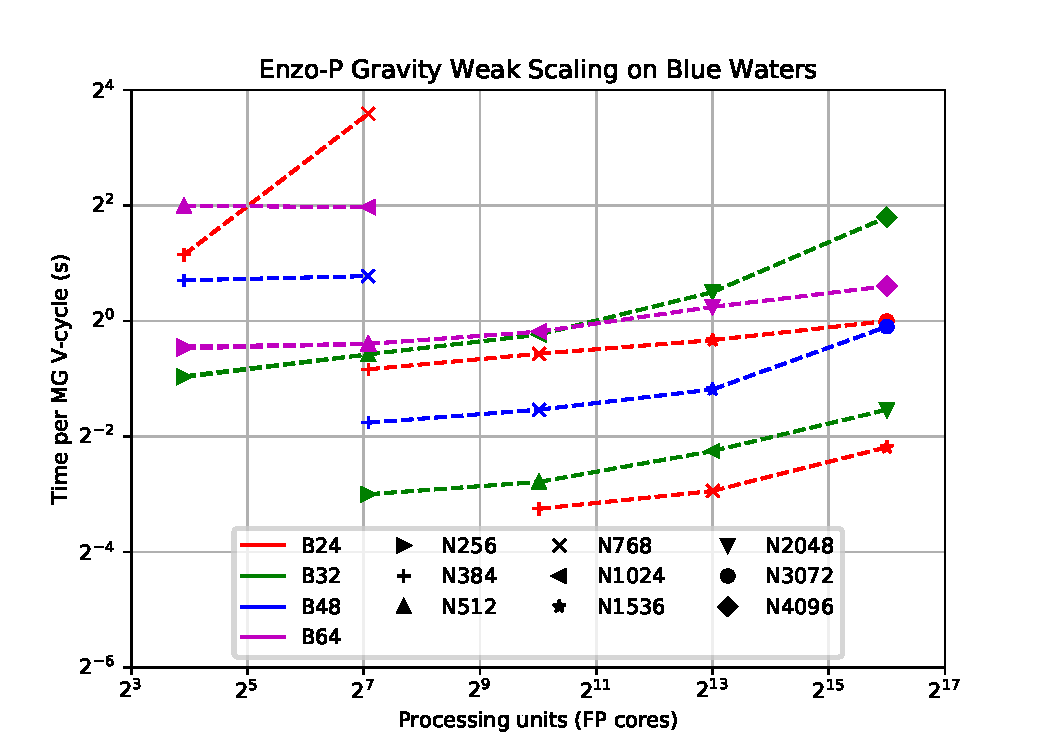
\includegraphics[width=4.0in]{scale-multigrid-weak.pdf}
        \end{minipage} \ 
      \end{center}
    \end{minipage}
  \end{center}
\end{frame}

\begin{frame}[fragile,label=ss-recent-gravity] 
\secframetitle{\ssRecentGravity}
\framesubtitle{Gravity strong scaling}
  \begin{center}
    \vspace{-0.1in}
    \begin{minipage}{4.5in}
      \begin{center}
        \begin{minipage}{4.0in}
          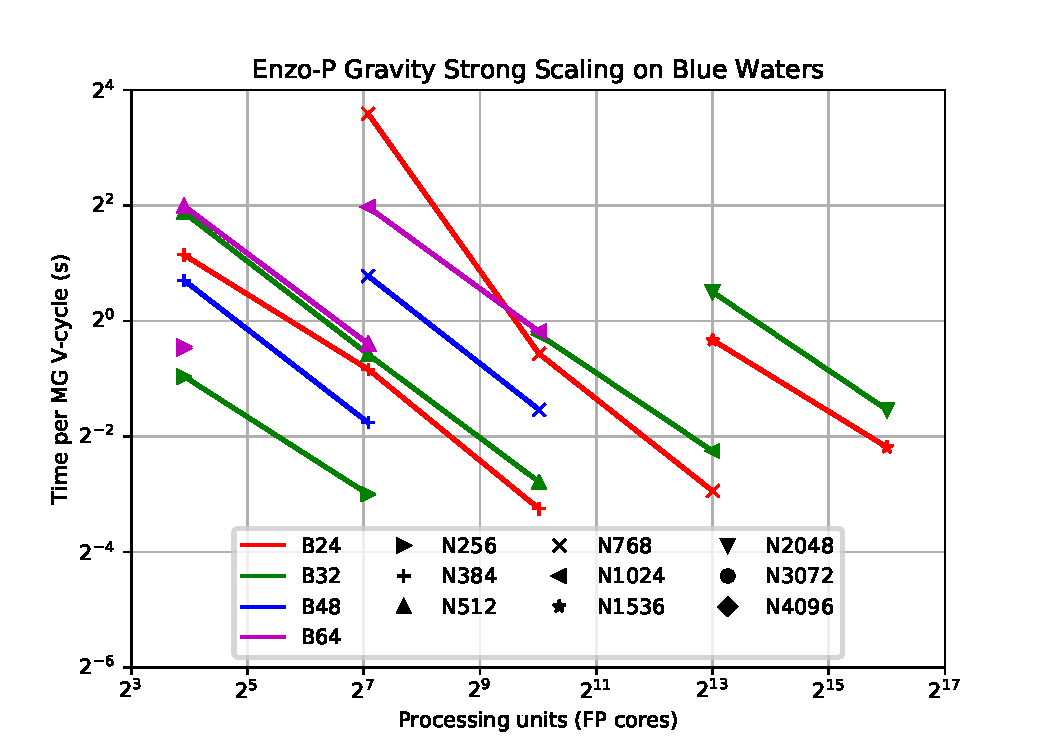
\includegraphics[width=4.0in]{scale-multigrid-strong.pdf}
        \end{minipage} \\
      \end{center}
    \end{minipage}
  \end{center}
\end{frame}

\begin{frame}[fragile,label=ss-recent-gravity] 
\secframetitle{\ssRecentGravity}
\framesubtitle{Projections view of one V-cycle ($P=8205$)}
  \begin{center}
    \vspace{-0.1in}
    \begin{minipage}{4.5in}
          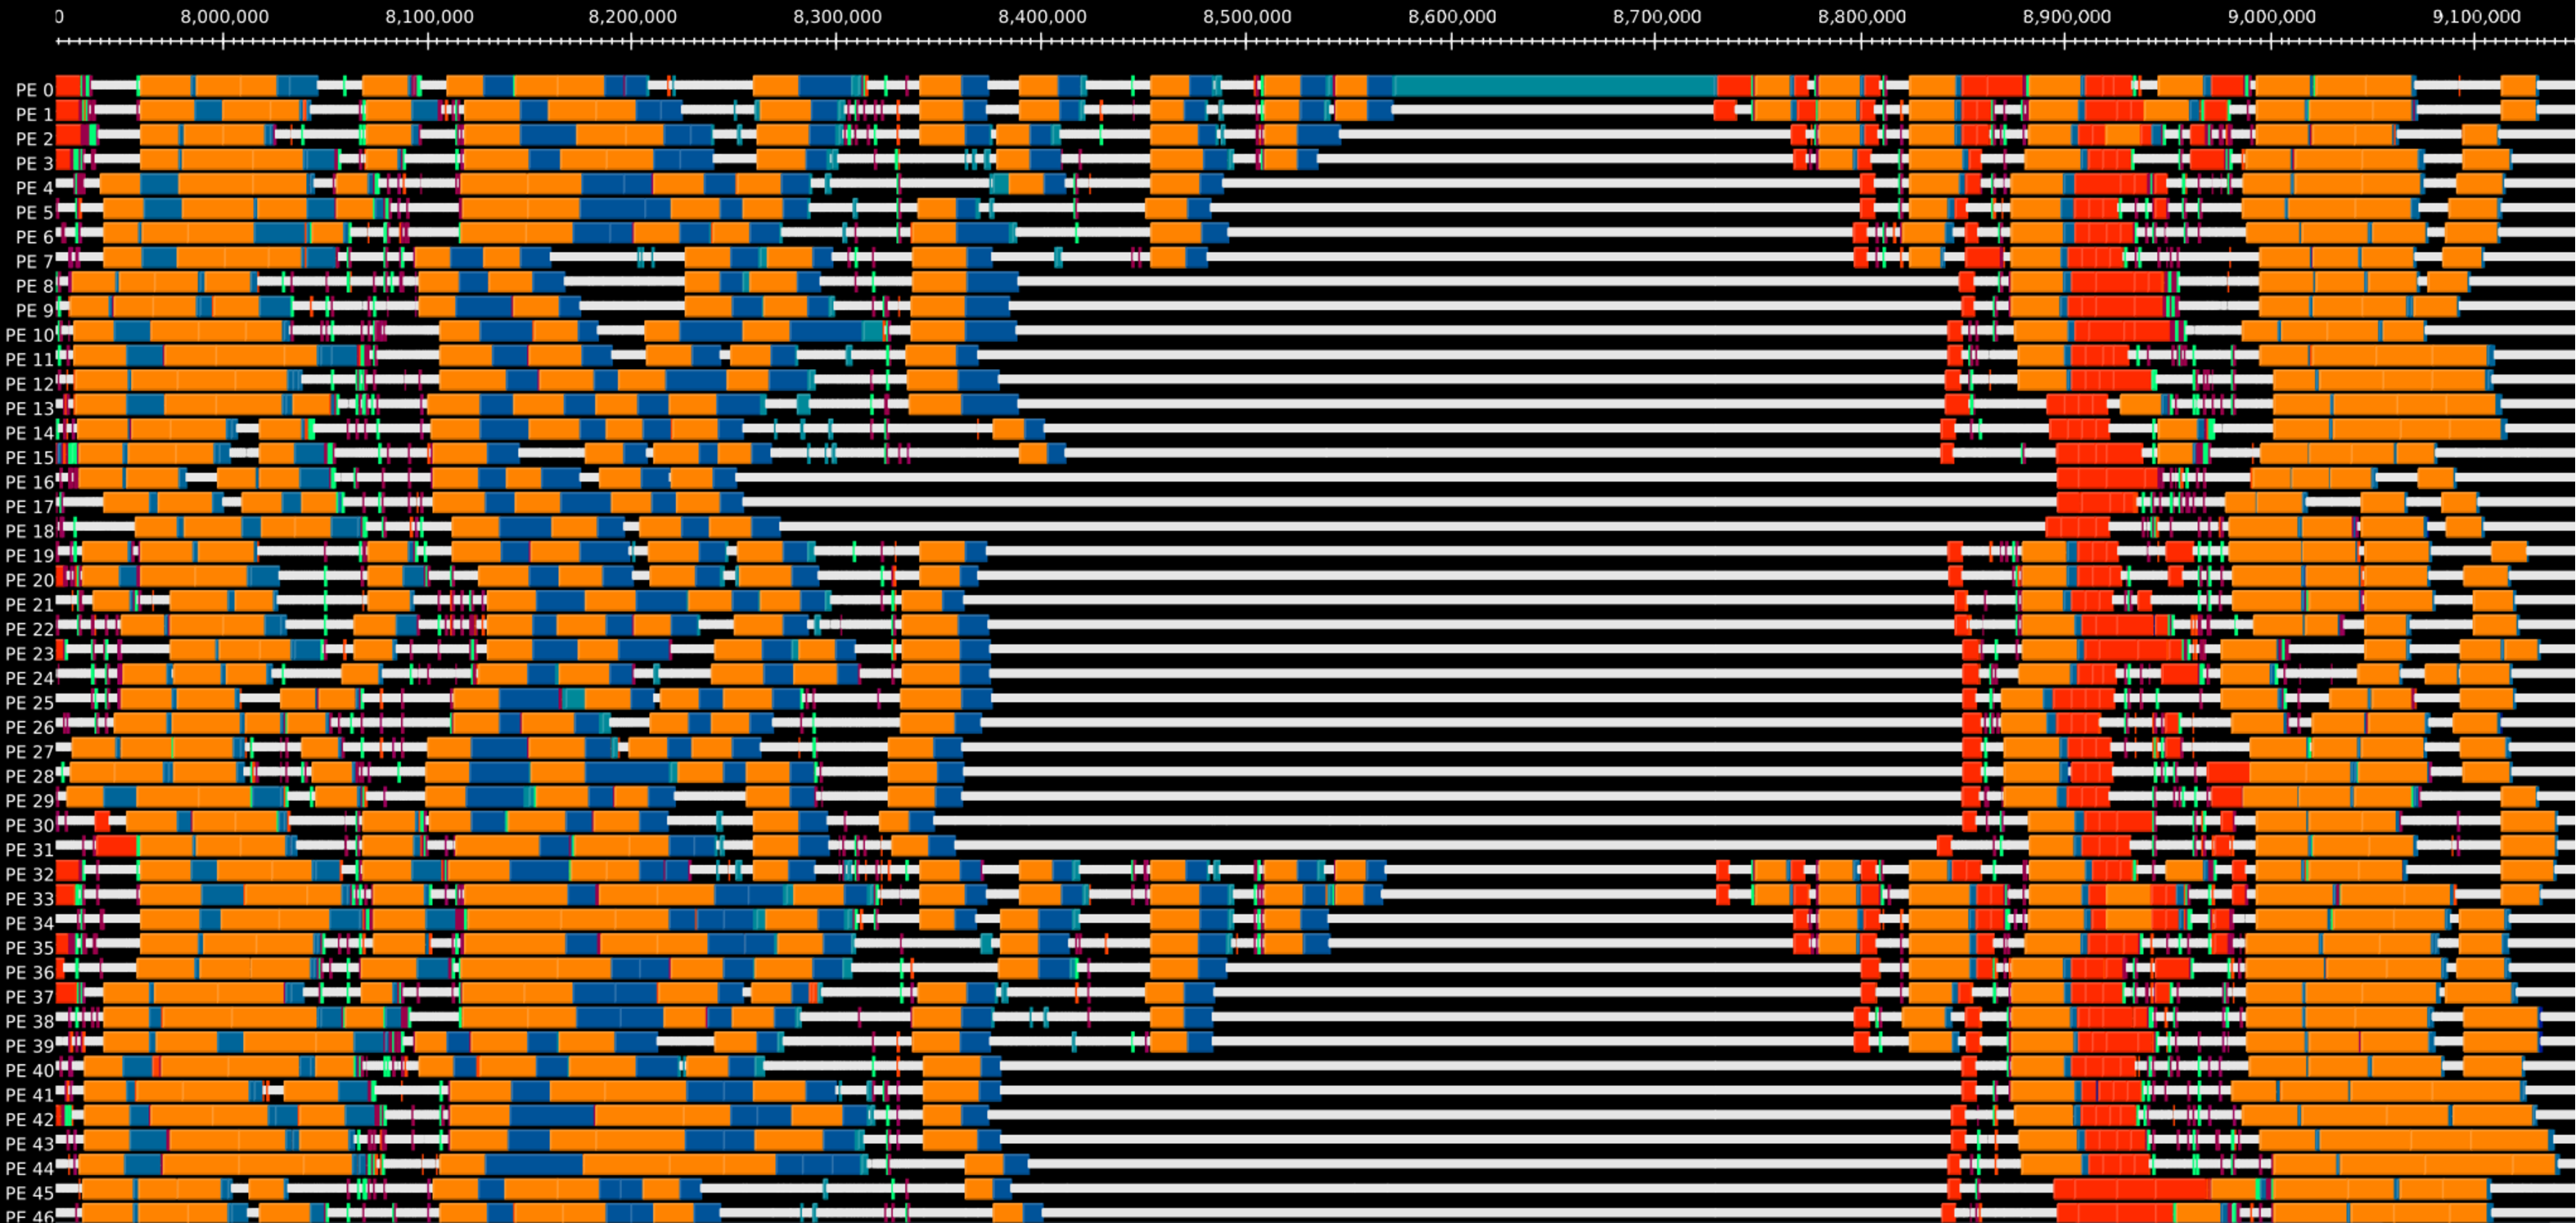
\includegraphics[width=4.5in]{mg0-vcycle-new-2.pdf}
    \end{minipage}
  \end{center}
\end{frame}
% 
%
%    [ IMAGE ] strong scaling
%    [ IMAGE ] weak scaling
%
%     Scalable through 64K
%
%     Projections visualization
%        P=8K
%
%        IMAGE: mg0-vcycle-old.pdf
%          non-scalable V-cycle
%          coarse grid problem--single block CG with global reductions
%        
%        IMAGE: mg0-vcycle-new.pdf
%          scalable V-cycle
%          coarse grid problem--single block CG on single process
%
%----------------------------------------------------------------------
%
\begin{frame}[fragile,label=ss-recent-gravity] 
\secframetitle{\ssRecentGravity}
\framesubtitle{Notes on gravity performance}
\begin{itemize}
\item Times are single MG V-cycle
\begin{itemize}
\item MG: $O(\log N)$ cycles
\end{itemize}
\item  How much to coarsen?
\begin{itemize}
\item tests go to single \code{Block}
\item coarse solver currently CG
\item could try single-Block MG0
\end{itemize}
\item Smaller blocks scale better
\begin{itemize}
\item  more blocks per process
\item better parallel efficiency in mid-levels
\item  but less efficient per block
\end{itemize}
\item Interleaving multiple solves could help
\end{itemize}
\end{frame}
%
%----------------------------------------------------------------------
%----------------------------------------------------------------------
% Scalable AMR Gravity
\begin{frame}[fragile,label=ss-recent-gravity] 
\secframetitle{\ssRecentGravity}
\framesubtitle{Mg0 V-cycle algorithm}
% Mg0: Multigrid solver for uniform grids
%
 I'm in level $0 < k < N$: what do I do?
 \begin{minipage}{2.5in}
\footnotesize
\vspace{0.1in}
\begin{tabbing}
\code{xxx}\=\code{xxx}\=\code{xxx}\=\kill
\>         1. do nothing (finer grids start) \\
\>         2. \bluetext{entry recv}: coarse residual from a child \\
\>\>	    2a. if not last child, do nothing \\
\>\>           2b. if last child, continue \\
\>         3. pre-smooth \\
\>         4. compute residual \\
\>	  5. \redtext{entry send}: coarse residual to parent \\
\>	  6. do nothing (coarser grids continue) \\
\>         7. \bluetext{entry recv}: correction from parent \\
\>         8. prolong correction and update solution \\
\>	  9. post-smooth \\
\>        10. \redtext{entry send}: correction to parent \\
\>\>           10a. if converged, end \\
\>\>	    10b. else goto 1
\end{tabbing}
\end{minipage}
\begin{minipage}{1.9in}
\centerline{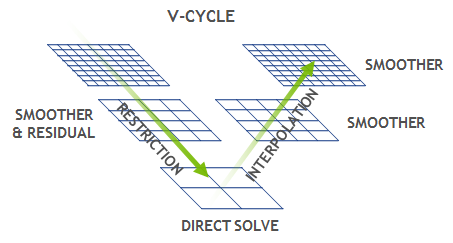
\includegraphics[width=2.0in]{hpgmg_v_cycle.png}}
\end{minipage}
\end{frame}
%
